\documentclass[11pt,a4paper]{article}
\usepackage[margin=2.2cm]{geometry}
\usepackage{amsmath,amssymb,amsthm}
\usepackage{booktabs}
\usepackage{graphicx}
\usepackage{hyperref}
\usepackage{xcolor}
\usepackage{enumitem}
\usepackage{tikz}
\usetikzlibrary{arrows.meta}
\setlist{nosep,leftmargin=1.4em}
\newtheorem{proposition}{Proposition}
\newcommand{\sgn}{\operatorname{sgn}}
\newcommand{\code}[1]{\texttt{#1}}

\title{Maximum positive regrasp for one 125\,ms gripper pulse\\[2pt]
\large Tilted Franka environment (\code{env\_franka\_parallel\_tilted.py})}
\author{Derivation behind \code{franka\_controllers/scripts/assess\_angle.py}}
\date{28 September 2026}

\begin{document}
\maketitle

\section*{Summary}
\begin{itemize}
  \item Section~\ref{sec:fbd} (page~\pageref{fig:fbd}) has the free-body diagram, all forces, and a step-by-step hand
        calculation with numbers.
  \item During the open window the block's position \emph{relative to the fingers}, $s$, obeys
        $\ddot s = -a_g - g\cos\theta - \mu g\sin\theta\,\sgn(\dot s)$. $s$ is exactly the change of the
        env's \code{cuboid\_rel\_z}.
  \item Under the env limits $|v_g|\le V=0.45$\,m/s and $|a_g|\le A=15$\,m/s$^2$, the best gripper motion
        (with no reliance on static friction) is \emph{bang-bang}. The gripper reaches the release moving up at $+V$,
        brakes at $-A$ for $t_1=\min(T,2V/A)=60$\,ms, then coasts at $-V$ for $t_2=T-t_1=65$\,ms.
        Its value $s^*(T)$ has the closed form of Section~\ref{sec:closed}.
  \item For $\theta=0$ the result is $s^*=8.86$\,mm for any $\mu$. For $\mu\in[0.05,0.3]$ it rises with tilt, up to
        16.4--28.6\,mm at $45^\circ$. At the env friction $\mu\in[0.6,0.9]$ and $\theta>0$ it falls to $\approx 0$--7\,mm
        and turns negative for $\mu\gtrsim0.75$ at $\theta\approx 20$--$35^\circ$.
  \item Static friction allows a small improvement (\emph{brake--catch--hold}, Section~\ref{sec:hold}):
        $\le0.3$\,mm for $\mu\le0.3$, but up to 4\,mm at $\mu=0.9$, where it makes the regrasp positive again.
        A free numerical optimiser over arbitrary profiles never beats this family.
  \item Timing matters. Each millisecond that braking starts \emph{before} the true release costs 0.8--1.0\,mm;
        each millisecond late costs 0.2--0.9\,mm.
  \item Optimising the parameters (Section~\ref{sec:opt}): $\partial s^*/\partial\mu<0$ for every $\theta>0$, so the best
        $\mu$ is the \emph{lowest} allowed. At $\mu=0.05$ that gives 17.33\,mm at $30^\circ$ and 28.60\,mm at $45^\circ$.
        For $\mu=0.05$ and $0.1$ the only point where $\partial s^*/\partial\theta=0$ is a \emph{minimum} (at $2.45^\circ$
        and $4.88^\circ$). The best tilt is therefore the upper limit, $\theta^*=45^\circ$: 28.60\,mm and 25.92\,mm.
  \item Acceleration limit at $45^\circ$, $\mu=0.05$ (Section~\ref{sec:accel}):
        $s^*=2V^2/b-\tfrac32V^2/A_{\rm brake}-\tfrac12V^2/A_{\rm rev}$ (minus a 0.007\,mm fall term).
        Raising $A$ from 12 to 20\,m/s$^2$ raises $s^*$ from 21.85 to 35.35\,mm. The \emph{braking} acceleration
        ($+V\to0$) is worth $3\times$ the \emph{reversing} one ($0\to-V$).
\end{itemize}

\section{What the environment fixes}
All positions and velocities are along the tilted grasp axis $\hat z$ ("task $z$"), with $+\hat z$ pointing up the axis.
The tilt $\theta$ is measured from world vertical and gravity stays world-down. The gravity component along $\hat z$
is therefore $-g\cos\theta$ and the component across it is $g\sin\theta$.

\begin{center}
\begin{tabular}{lll}
\toprule
Quantity & Value & Source in env \\
\midrule
Velocity limit $V$ & 0.45 m/s & \code{Z\_VEL\_MAX} \\
Acceleration limit $A$ & 15 m/s$^2$ & \code{Z\_ACC\_MAX}, $|\Delta v|\le A\,\Delta$ per step \\
Control period $\Delta$ & 20 ms & \code{target\_dt} \\
Block & $25\times25\times150$ mm, 35 g & \code{box.xml} \\
Contact friction & 0.6--0.9 (randomised) & \code{FRICTION\_MIN/MAX} \\
Free time of the block $T$ & 125 ms (your value) & pulse: 2 delay + 6 open + 1 close steps \\
Measured quantity & \code{cuboid\_rel\_z} & block centre $-$ fingertip midpoint, along $\hat z$ \\
\bottomrule
\end{tabular}
\end{center}

\paragraph{The acceleration really is piecewise constant.}
Each step updates the velocity target $v_0\to v_1$ with $|v_1-v_0|\le A\Delta$ and advances the position with the
trapezoid rule, $z_1=z_0+\tfrac12(v_0+v_1)\Delta$. The 1\,kHz reference is then the cubic Hermite curve through
$(z_0,v_0)$ and $(z_1,v_1)$. Differentiating the Hermite basis and substituting the trapezoid relation gives
\[
  v(\sigma) = 6(\sigma-\sigma^2)\tfrac{z_1-z_0}{\Delta} + (3\sigma^2-4\sigma+1)v_0 + (3\sigma^2-2\sigma)v_1
            = (1-\sigma)\,v_0 + \sigma\,v_1 ,\qquad \sigma\in[0,1].
\]
So the reference velocity is linear inside every step and the reference acceleration is the constant $(v_1-v_0)/\Delta$,
with $|a|\le A$. Braking from $+V$ to $-V$ takes exactly three steps of $\Delta v=-0.3$\,m/s (60\,ms).
The model below treats the reference as the true gripper motion. The velocity feed-forward filter
($\omega_n=75$\,rad/s, $\zeta=0.33$) and the IK tracking are ignored (see Section~\ref{sec:assump}).

\section{Relative motion of the free block}
Let $z_g(t)$ be the gripper (fingertip midpoint) and $z_b(t)$ the block, both along $\hat z$. Time $t=0$ is the
moment the grip force is gone (the env's own marker: average finger force $<0.15$\,N). Time $t=T$ is the moment the
block is gripped again ($\ge0.75$\,N). Define
\[
  s(t) = z_b(t)-z_g(t) - \big(z_b(0)-z_g(0)\big), \qquad u=\dot s .
\]
Then $s(T)$ is exactly the change of \code{cuboid\_rel\_z} over the pulse. The block was held until $t=0$, so
$s(0)=0$ and $u(0)=0$.

While the fingers are open the block leans on the lower finger. The gripper accelerates only along $\hat z$, so the
normal load is $N=mg\sin\theta$ and the Coulomb friction force is bounded by $c\,m$ with $c:=\mu g\sin\theta$.
In the gripper frame (pseudo-force $-m a_g$):
\begin{equation}
  \ddot s = \underbrace{-a_g(t) - g\cos\theta}_{=:F(t)\ \text{(drive)}} - c\,\sgn(u),
  \qquad
  \text{and if } u=0,\ |F|\le c: \ \text{the block sticks } (\ddot s=0).
  \label{eq:eom}
\end{equation}
Write $g_a:=g\cos\theta$. The block can \emph{break upward} from rest only if $F>c$, i.e.\ $-a_g>g_a+c$.
The strongest available drive is $a_g=-A$, so
\begin{equation}
  \boxed{\text{upward motion is possible at all}\iff A > g(\cos\theta+\mu\sin\theta).}
  \label{eq:feas}
\end{equation}
For $\theta\le45^\circ$ and $\mu\le0.9$ the right side is at most $13.2$\,m/s$^2<15$, so this always holds.
In this range, "no positive regrasp" means the block rises and then falls back below its start before $T$.

% Free-body diagram and hand-calculation sheet (\input by regrasp_pulse_math.tex)
\section{Free-body diagram and hand calculation}\label{sec:fbd}
This section contains everything needed to redo the result by hand: the forces on the block, the equation of
motion in both frames, and a phase-by-phase calculation with numbers. Symbols:
$m=0.035$\,kg, $g=9.81$\,m/s$^2$, tilt $\theta$, friction $\mu$, speed limit $V$, braking/reversing accelerations
$A_{\rm b}$, $A_{\rm r}$, and free time $T$. $\hat z$ is the grasp axis (positive up the axis) and $\hat x$ is
perpendicular to it in the tilt plane, pointing away from the lower finger.

\begin{figure}[h]
\centering
\resizebox{\linewidth}{!}{%
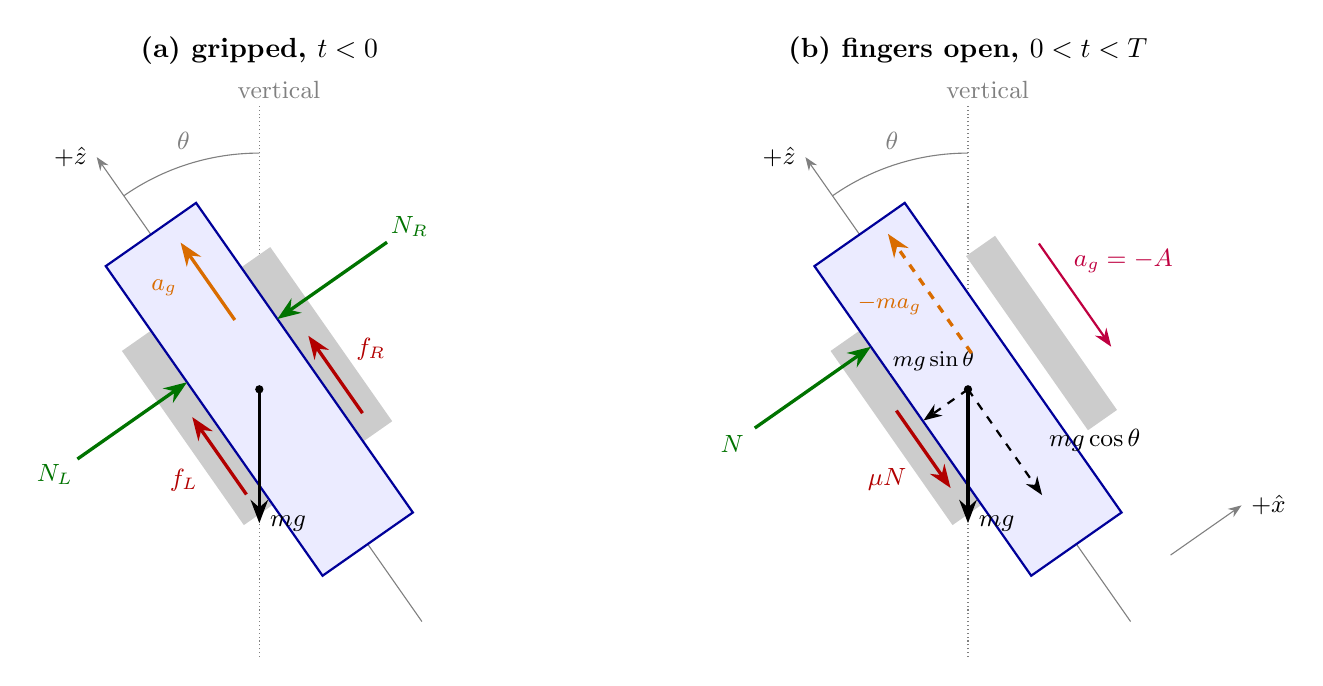
\begin{tikzpicture}[>=Stealth, every node/.style={font=\small}]
  % ================= (a) gripped =================
  \begin{scope}
    \node[font=\normalsize\bfseries] at (0,4.3) {(a) gripped, $t<0$};
    \draw[densely dotted, gray] (0,-3.4) -- (0,3.6);
    \node[gray] at (0.25,3.8) {vertical};
    \begin{scope}[rotate=35]
      \draw[->, gray] (0,-3.6) -- (0,3.6) node[left, text=black]{$+\hat z$};
      \fill[gray!40] (-1.15,-1.3) rectangle (-0.7,1.4);
      \fill[gray!40] (0.7,-1.3) rectangle (1.15,1.4);
      \filldraw[fill=blue!8, draw=blue!60!black, thick] (-0.7,-2.4) rectangle (0.7,2.4);
      \draw[->, very thick, green!45!black] (-2.4,0.6) -- (-0.7,0.6);
      \node[green!45!black] at (-2.75,0.6) {$N_L$};
      \draw[->, very thick, green!45!black] (2.4,0.6) -- (0.7,0.6);
      \node[green!45!black] at (2.75,0.6) {$N_R$};
      \draw[->, very thick, red!70!black] (-0.9,-1.0) -- (-0.9,0.2);
      \node[red!70!black] at (-1.45,-0.4) {$f_L$};
      \draw[->, very thick, red!70!black] (0.9,-1.0) -- (0.9,0.2);
      \node[red!70!black] at (1.45,-0.4) {$f_R$};
      \draw[->, very thick, orange!85!black] (0.25,0.9) -- (0.25,2.1);
      \node[orange!85!black] at (-0.25,1.75) {$a_g$};
    \end{scope}
    \draw[->, very thick] (0,0) -- (0,-1.7) node[right]{$mg$};
    \fill (0,0) circle (1.5pt);
    \draw[gray] (0,3.0) arc (90:125:3.0);
    \node[gray] at ({3.3*cos(107)},{3.3*sin(107)}) {$\theta$};
  \end{scope}
  % ================= (b) open =================
  \begin{scope}[shift={(9,0)}]
    \node[font=\normalsize\bfseries] at (0,4.3) {(b) fingers open, $0<t<T$};
    \draw[densely dotted, gray] (0,-3.4) -- (0,3.6);
    \node[gray] at (0.25,3.8) {vertical};
    \begin{scope}[rotate=35]
      \draw[->, gray] (0,-3.6) -- (0,3.6) node[left, text=black]{$+\hat z$};
      \draw[->, gray] (0.9,-3.2) -- (2.0,-3.2) node[right, text=black]{$+\hat x$};
      \fill[gray!40] (-1.15,-1.3) rectangle (-0.7,1.4);            % lower finger (contact)
      \fill[gray!40] (0.95,-1.3) rectangle (1.4,1.4);              % upper finger (gap exaggerated)
      \draw[->, thick, purple] (1.8,1.0) -- (1.8,-0.6);
      \node[purple] at (2.55,0.2) {$a_g=-A$};
      \filldraw[fill=blue!8, draw=blue!60!black, thick] (-0.7,-2.4) rectangle (0.7,2.4);
      % normal
      \draw[->, very thick, green!45!black] (-2.5,1.15) -- (-0.7,1.15);
      \node[green!45!black] at (-2.85,1.15) {$N$};
      % kinetic friction (u > 0)
      \draw[->, very thick, red!70!black] (-0.9,0.3) -- (-0.9,-0.9);
      \node[red!70!black] at (-1.5,-0.35) {$\mu N$};
      % gravity components
      \draw[->, dashed, thick] (0,0) -- (0,-1.64);
      \node at (0.95,-1.45) {$mg\cos\theta$};
      \draw[->, dashed, thick] (0,0) -- (-1.15*0.6,0);
      \node[fill=blue!8, inner sep=1pt] at (-0.15,0.55) {\footnotesize$mg\sin\theta$};
      % inertial force (gripper frame)
      \draw[->, very thick, dashed, orange!85!black] (0.3,0.35) -- (0.3,2.2);
      \node[orange!85!black, fill=blue!8, inner sep=1pt] at (-0.2,1.45) {\footnotesize$-m a_g$};
    \end{scope}
    \draw[->, very thick] (0,0) -- (0,-1.7) node[right]{$mg$};
    \fill (0,0) circle (1.5pt);
    \draw[gray] (0,3.0) arc (90:125:3.0);
    \node[gray] at ({3.3*cos(107)},{3.3*sin(107)}) {$\theta$};
  \end{scope}
\end{tikzpicture}}
\caption{Forces on the block (grey: finger pads; the grasp axis $+\hat z$ is tilted $\theta$ from vertical).
(a) Gripped: squeeze normals $N_L,N_R$ and static friction $f_L,f_R$ on both faces; the block moves with the gripper
acceleration $a_g$. (b) Fingers open: the block leans on the lower finger, which pushes back with normal $N$. Kinetic
friction $\mu N$ opposes the relative sliding. It is drawn for the block sliding \emph{up} the fingers ($u>0$), and it
points up the axis once the block slides back down. Dashed black: the components of $mg$. Dashed orange: the inertial
force $-ma_g$, which only appears when you write the equations in the gripper frame. The 1\,mm gap to the upper
finger is exaggerated.}
\label{fig:fbd}
\end{figure}

\subsection*{Forces while the fingers are open (b)}
There is no acceleration across the axis (the transverse controller holds the line), so the $\hat x$ balance gives
the normal load. The $\hat z$ balance then gives the motion.
\begin{center}
\small
\begin{tabular}{llll}
\toprule
Force & direction & magnitude & value at $45^\circ$, $\mu=0.05$\\
\midrule
weight $mg$ & world down & $mg$ & 0.3434 N\\
\quad along axis & $-\hat z$ & $mg\cos\theta$ & 0.2428 N\\
\quad across axis & $-\hat x$ (into lower finger) & $mg\sin\theta$ & 0.2428 N\\
normal $N$ & $+\hat x$ & $N=mg\sin\theta$ & 0.2428 N\\
friction & $-\sgn(u)\,\hat z$ & $\mu N=\mu mg\sin\theta$ & 0.01214 N\\
inertial (gripper frame only) & $-a_g$ direction & $m|a_g|$ & $0.525$ N at $A=15$\\
\bottomrule
\end{tabular}
\end{center}
\begin{align*}
  \text{across the axis:}\quad & N - mg\sin\theta = 0 \ \Rightarrow\ N=mg\sin\theta,\\[2pt]
  \text{along, world frame:}\quad & m\,\ddot z_b = -mg\cos\theta - \mu N\,\sgn(u),\\
  & \ddot z_b=-b=-g(\cos\theta+\mu\sin\theta)\ \ \text{if } u>0\ \text{(block sliding up the fingers)},\\
  & \ddot z_b=-d=-g(\cos\theta-\mu\sin\theta)\ \ \text{if } u<0\ \text{(sliding back down)},\\[2pt]
  \text{along, gripper frame:}\quad & m\,\ddot s = -mg\cos\theta - \mu N\,\sgn(u) - m a_g,\\
  & \ddot s = -a_g - b\ \ (u>0),\qquad \ddot s=-a_g-d\ \ (u<0).
\end{align*}
The displacement you want is always
\[
  s(T)=\Delta z_b-\Delta z_g=\int_0^T\big(v_b(t)-v_g(t)\big)\,dt
  \qquad\text{(area between the block and gripper velocity lines).}
\]
\emph{Stick check:} if $u=0$, the block stays put as long as $|{-a_g}-g\cos\theta|\le\mu g\sin\theta$.

\subsection*{Forces while gripped (a)}
The block has the gripper's acceleration $a_g$. Along the axis
$f_L+f_R=m(g\cos\theta+a_g)$ and across $N_L-N_R=mg\sin\theta$. Static friction must not slip,
$f_L+f_R\le\mu(N_L+N_R)\approx2\mu N_{\rm grip}$. The worst case is the pre-release acceleration up to $+V$ at
$a_g=+A$:
\[
  N_{\rm grip}\ \ge\ \frac{m\,(g\cos\theta+A)}{2\mu}\;=\;7.68\ \text{N}\ (A=15),\qquad 9.43\ \text{N}\ (A=20)
  \qquad(45^\circ,\ \mu=0.05).
\]

\subsection*{Step-by-step calculation}
Take the gripper profile of Section~\ref{sec:closed}. At release the gripper moves up at $+V$. It brakes to 0 at
$-A_{\rm b}$, reverses to $-V$ at $-A_{\rm r}$, then coasts. The block keeps sliding up the fingers ($u>0$) until
$t_p$, so its world acceleration is the constant $-b$ until then.
\begin{center}
\small
\renewcommand{\arraystretch}{1.25}
\begin{tabular}{p{3.2cm}p{6.1cm}rr}
\toprule
Step & formula & $A=15$ & $A=20$\\
\midrule
0. constants & $b=g(\cos\theta+\mu\sin\theta)$ [m/s$^2$] & 7.2836 & 7.2836\\
 & $d=g(\cos\theta-\mu\sin\theta)$ [m/s$^2$] & 6.5899 & 6.5899\\
1. braking $+V\to0$ & $t_a=V/A_{\rm b}$ & 30.000 ms & 22.500 ms\\
 & $\ddot s=A_{\rm b}-b$ [m/s$^2$] & 7.7164 & 12.7164\\
 & $u_1=(A_{\rm b}-b)t_a$ & 0.23149 m/s & 0.28612 m/s\\
 & $s_1=\tfrac12(A_{\rm b}-b)t_a^2$ & 3.4724 mm & 3.2189 mm\\
2. reversing $0\to-V$ & $t_r=V/A_{\rm r}$, \ $\ddot s=A_{\rm r}-b$ & 30.000 ms & 22.500 ms\\
 & $u_2=u_1+(A_{\rm r}-b)t_r$ & 0.46299 m/s & 0.57224 m/s\\
 & $s_2=s_1+u_1t_r+\tfrac12(A_{\rm r}-b)t_r^2$ & 13.8896 mm & 12.8754 mm\\
3. coast to the peak & $\ddot s=-b$, \ $t_s=u_2/b$ & 63.566 ms & 78.566 ms\\
 & $t_p=t_a+t_r+t_s$ \ (must be $<T$) & 123.566 ms & 123.566 ms\\
 & $s_p=s_2+u_2^2/(2b)$ & 28.6047 mm & 35.3547 mm\\
4. fall back & $r=T-t_p$, \ $\ddot s=-d$ & 1.4339 ms & 1.4339 ms\\
 & $\tfrac12 d\,r^2$ & 0.0068 mm & 0.0068 mm\\
\midrule
\textbf{result} & $s(T)=s_p-\tfrac12 d r^2$ & \textbf{28.598 mm} & \textbf{35.348 mm}\\
\bottomrule
\end{tabular}
\end{center}
If $t_p\ge T$, stop at step 3 with $s(T)=s_2+u_2(T-t_a-t_r)-\tfrac12 b(T-t_a-t_r)^2$. If $d\le0$, skip step 4,
because the block sticks at the peak.

\paragraph{Cross-check in the world frame.} Compute the two displacements separately and subtract.
The gripper covers a triangle during braking, a triangle during reversing, and a rectangle while coasting:
\[
  \Delta z_g = \tfrac12Vt_a-\tfrac12Vt_r-V(T-t_a-t_r) = -VT+\frac{3V^2}{2A_{\rm b}}+\frac{V^2}{2A_{\rm r}} .
\]
The block decelerates at $b$ from $+V$ to $-V$ until $t_p$, then at $d$:
\[
  \Delta z_b = \big(Vt_p-\tfrac12 b\,t_p^2\big)-\big(Vr+\tfrac12 d\,r^2\big),\qquad s(T)=\Delta z_b-\Delta z_g .
\]
\begin{center}
\small
\begin{tabular}{lrr}
\toprule
 & $A=15$ & $A=20$\\
\midrule
$\Delta z_g$ (gripper) & $-29.250$ mm & $-36.000$ mm\\
$\Delta z_b$ (block) & $-0.652$ mm & $-0.652$ mm\\
$s(T)=\Delta z_b-\Delta z_g$ & 28.598 mm & 35.348 mm\\
\bottomrule
\end{tabular}
\end{center}
Once released, the block moves the same way for every $A$: it goes up, comes back, and ends 0.65\,mm below where it
was released. The regrasp comes \emph{entirely} from how far the gripper travels down in the same time.

\begin{figure}[h]
\centering
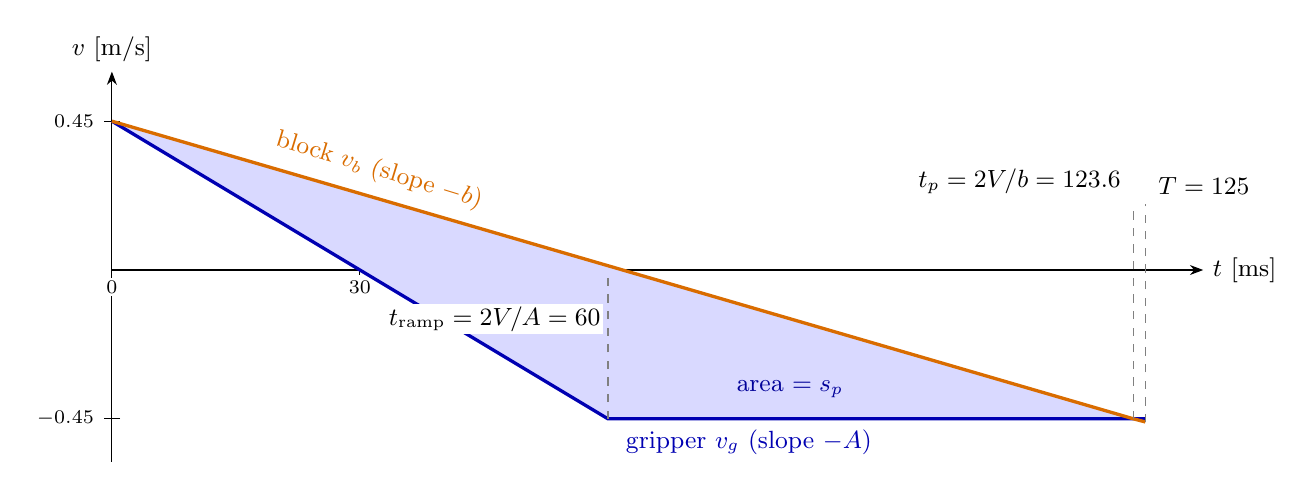
\begin{tikzpicture}[>=Stealth, x=0.105cm, y=4.2cm, every node/.style={font=\small}]
  % axes
  \draw[->] (0,0) -- (132,0) node[right]{$t$ [ms]};
  \draw[->] (0,-0.58) -- (0,0.6) node[above]{$v$ [m/s]};
  \foreach \t in {0,30} \draw (\t,0.015) -- (\t,-0.015) node[below=1pt, fill=white, inner sep=1pt]{\scriptsize\t};
  \foreach \v in {-0.45,0.45} \draw (1,\v) -- (-1,\v) node[left]{\scriptsize$\v$};
  % shaded area = s
  \fill[blue!15] (0,0.45) -- (123.566,-0.45) -- (60,-0.45) -- cycle;
  \fill[red!20] (123.566,-0.45) -- (125,-0.4594) -- (125,-0.45) -- cycle;
  % gripper velocity
  \draw[very thick, blue!70!black] (0,0.45) -- (60,-0.45) -- (125,-0.45);
  \node[blue!70!black, anchor=west] at (61,-0.52) {gripper $v_g$ (slope $-A$)};
  % block velocity
  \draw[very thick, orange!85!black] (0,0.45) -- (123.566,-0.45) -- (125,-0.4594);
  \node[orange!85!black, anchor=south west, rotate=-17] at (18,0.34) {block $v_b$ (slope $-b$)};
  % markers
  \draw[dashed, gray] (60,-0.45) -- (60,0);
  \node[anchor=north east, fill=white, inner sep=1pt] at (59.5,-0.1) {$t_{\rm ramp}=2V/A=60$};
  \draw[dashed, gray] (123.566,-0.45) -- (123.566,0.2);
  \node[anchor=south east] at (123.2,0.2) {$t_p=2V/b=123.6$};
  \draw[dashed, gray] (125,-0.46) -- (125,0.2);
  \node[anchor=south west] at (125.4,0.2) {$T=125$};
  \node[blue!60!black] at (82,-0.36) {area $=s_p$};
\end{tikzpicture}
\caption{Velocities along the axis for $A_{\rm b}=A_{\rm r}=15$ (the $\theta=45^\circ$, $\mu=0.05$ example). The
relative displacement is the area between the block and the gripper lines. Up to the peak this area is a triangle
with height $2V$ and base $t_p-t_{\rm ramp}$, so $s_p=V(t_p-t_{\rm ramp})=0.45\times(123.566-60)$\,ms $=28.605$\,mm.
The tiny red sliver after $t_p$ is the fall-back, $0.007$\,mm. A larger $A$ makes the ramp steeper and the triangle
wider; $t_p$ does not move.}
\label{fig:vel}
\end{figure}

\paragraph{Quick formulas to check against.}
\begin{gather*}
  t_p=\frac{2V}{b},\qquad
  s(T)=\frac{2V^2}{b}-\frac{3V^2}{2A_{\rm b}}-\frac{V^2}{2A_{\rm r}}-\tfrac12 d\,(T-t_p)^2,\\
  \text{equal limits } A_{\rm b}=A_{\rm r}=A:\quad s(T)=V\Big(\frac{2V}{b}-\frac{2V}{A}\Big)-\tfrac12 d\,(T-t_p)^2 .
\end{gather*}

\paragraph{Where the pulse fires in the env.}
Figure~\ref{fig:timeline} places the example on the env's 20\,ms control grid.
\begin{itemize}
  \item The policy \emph{triggers} the pulse at step $k$ by moving the finger action through the midpoint.
  \item Steps $k$ and $k+1$ are the 40\,ms delay, during which the policy's own finger command applies.
  \item Steps $k+2$ to $k+7$ force the fingers fully open (120\,ms), and step $k+8$ forces them closed.
\end{itemize}
The block only comes loose once a finger opens past the block's half width (12.5\,mm of the 13\,mm stroke), so in
practice that is when the forced-open window starts. Your $T=125$\,ms free time matches this: 120\,ms forced open
plus about 5\,ms for the fingers to close back onto the block. \textbf{Assumption:} the release is at the start of
step $k+2$ and the policy does not command fully open during the delay. If it does, the block is released up to
40\,ms earlier and the free time grows to about 165\,ms.

The gripper velocity targets that realise the optimum, one per 20\,ms step ($\Delta v\le A\cdot20$\,ms $=0.3$\,m/s):
\begin{center}
\small
\resizebox{\linewidth}{!}{%
\begin{tabular}{l|ccccccccccc}
\toprule
step & $k-2$ & $k-1$ & $k$ & $k+1$ & $k+2$ & $k+3$ & $k+4$ & $k+5\dots k+7$ & $k+8$ & $k+9$ & $k+10$\\
\midrule
$v$ target [m/s] (end of step) & 0.30 & 0.45 & 0.45 & 0.45 & 0.15 & $-0.15$ & $-0.45$ & $-0.45$ & $-0.45$ & $-0.15$ & 0\\
fingers & \multicolumn{2}{c}{gripped} & \multicolumn{2}{c}{delay} & \multicolumn{5}{c}{open (block free)} & \multicolumn{2}{c}{gripped}\\
\bottomrule
\end{tabular}}
\end{center}
The gripper is at $+V$ \emph{before} the trigger, holds it through the delay, and starts braking on exactly the step
where the fingers let go. The brake takes 3 steps ($+0.45\to0.15\to-0.15\to-0.45$). The gripper then coasts at $-V$
until the block is re-gripped, and only then decelerates to rest. Timing matters: starting the brake one step
(20\,ms) \emph{early}, while the block is still gripped, drops $s(T)$ from 28.6 to 6.7\,mm. Starting it one step
\emph{late} drops it to 13.2\,mm.

\begin{figure}[h]
  \centering
  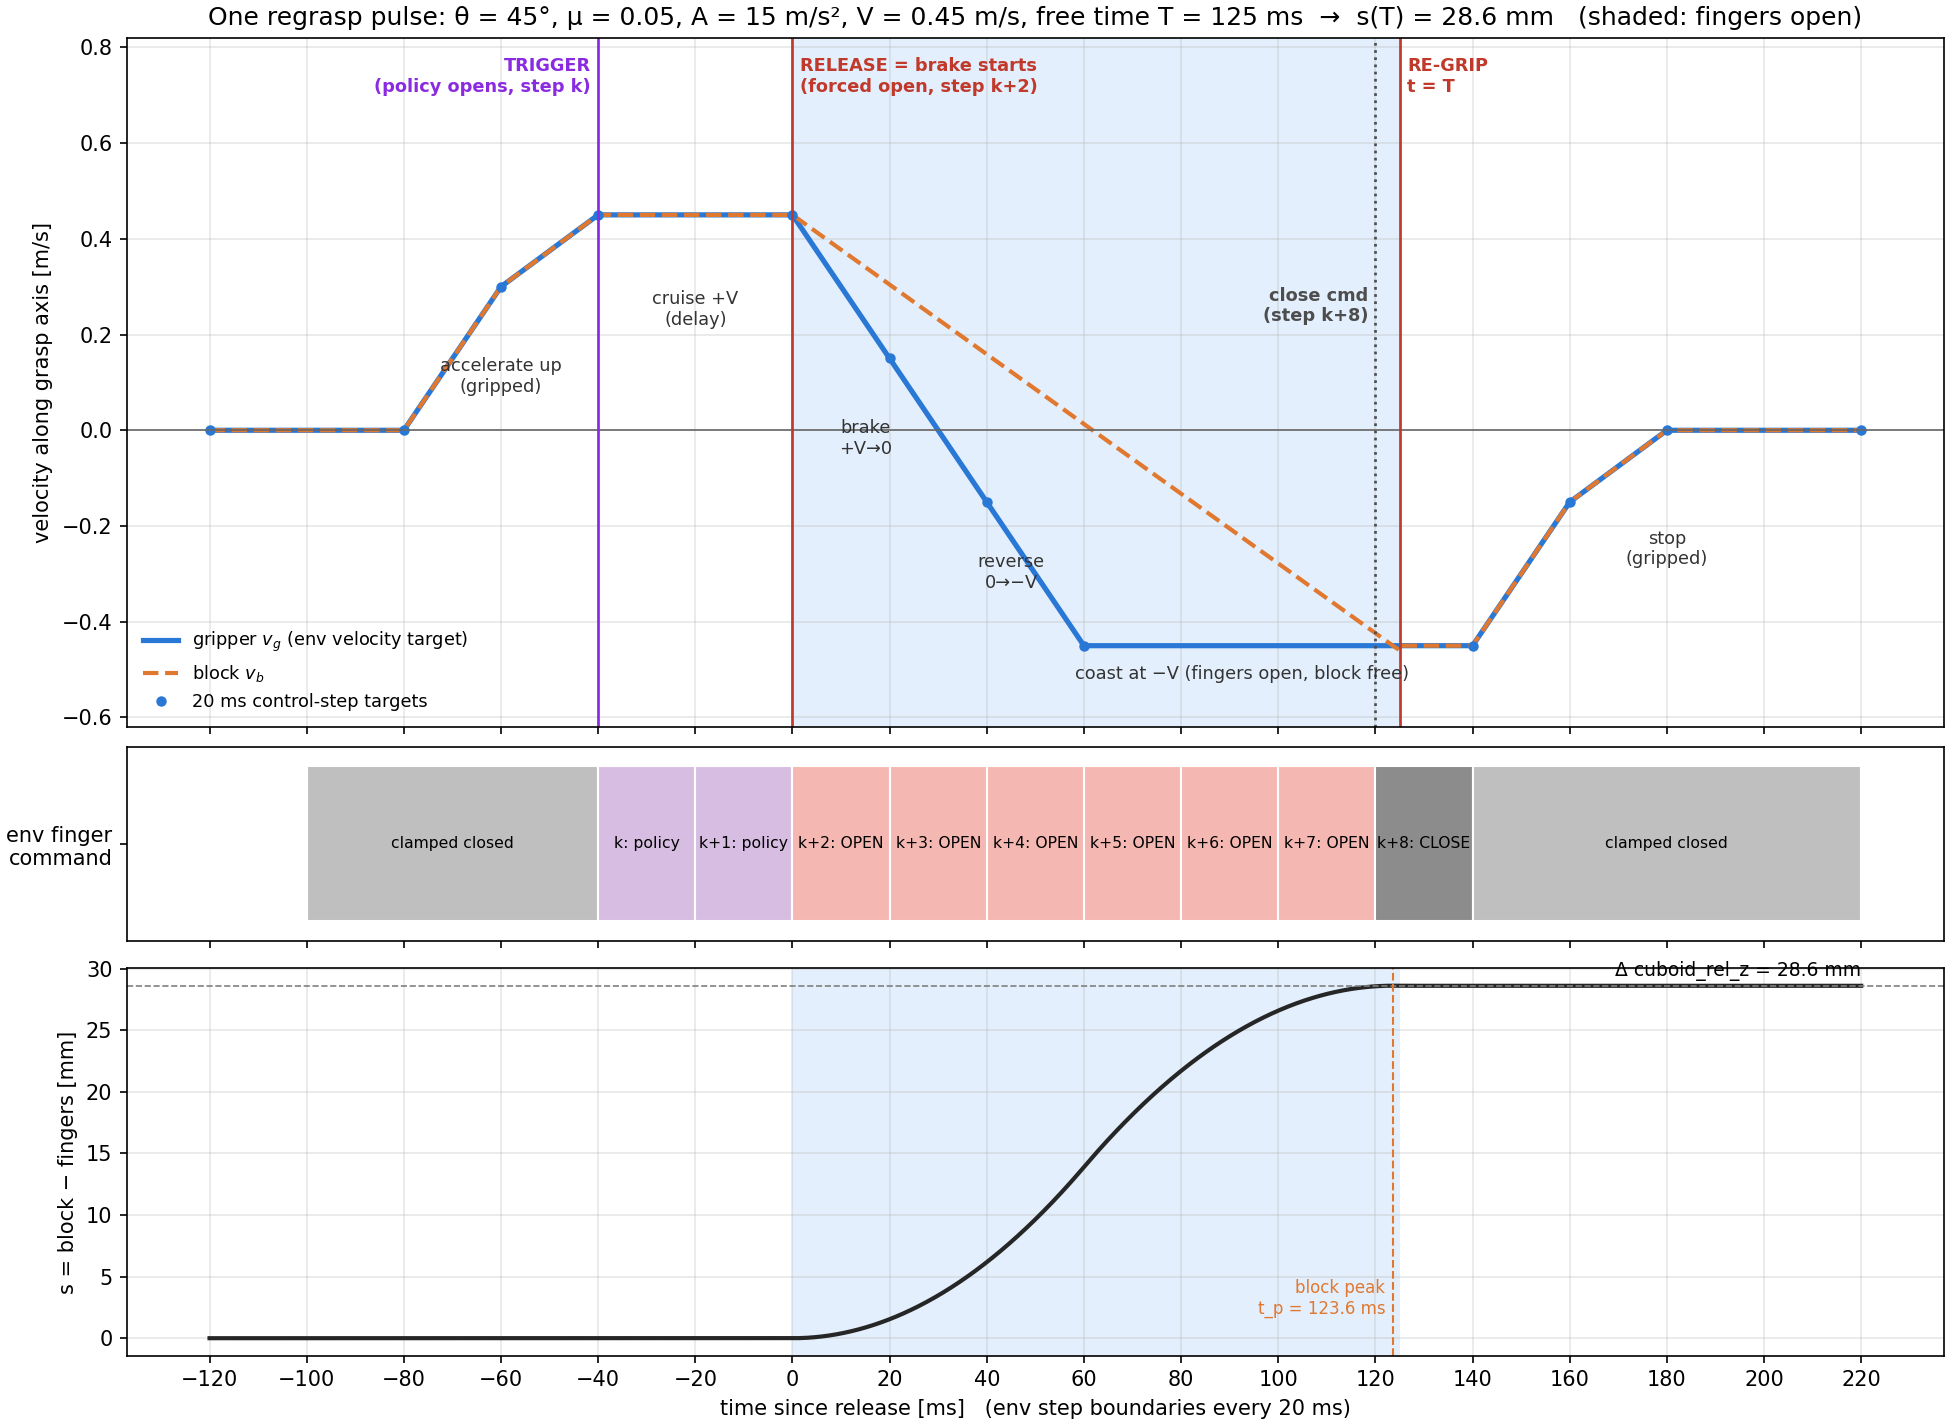
\includegraphics[width=\linewidth]{fig_timeline.png}
  \caption{One pulse for $\theta=45^\circ$, $\mu=0.05$, $A=15$\,m/s$^2$, $V=0.45$\,m/s, $T=125$\,ms. Top: gripper
  (blue) and block (orange) velocity along the axis. They coincide while gripped and separate in the shaded open
  window. The area between them is the regrasp. Middle: the env's finger command per 20\,ms step, relative to the
  trigger step $k$. Bottom: the block's displacement in the fingers, which ends at $+28.6$\,mm.}
  \label{fig:timeline}
\end{figure}


\section{The optimisation problem}
\begin{equation}
  \max_{a_g(\cdot),\,v_g(0)}\ s(T)\quad\text{s.t.}\quad \eqref{eq:eom},\ \ |a_g(t)|\le A,\ \ |v_g(t)|\le V,\ \ s(0)=u(0)=0 .
  \label{eq:ocp}
\end{equation}
The gripper position does not appear, and $v_g(0)$ is free: the gripper can build up speed while it still holds the block.

\begin{proposition}[frictionless and rising-only case]\label{prop:bb}
Integrate \eqref{eq:eom} twice. If $\sgn(u)$ is constant $=+1$ on $[0,T]$ (the block never falls back), or $c=0$, then
\begin{equation}
  s(T) = -\tfrac12 (g_a + c)\,T^2 + \int_0^T \big(v_g(0)-v_g(t)\big)\,dt .
  \label{eq:identity}
\end{equation}
The integral is maximised by $v_g(0)=V$ and $v_g(t)=\max(V-At,\,-V)$. This is the \emph{bang-bang} profile:
brake at $-A$ for $t_1=2V/A$, then coast at $-V$.
\end{proposition}
\begin{proof}
$\ddot s = -a_g-g_a-c$, and $\int_0^T\!\int_0^t a_g\,d\tau\,dt=\int_0^T(v_g(t)-v_g(0))\,dt$, which gives
\eqref{eq:identity}. Any admissible profile satisfies $v_g(0)\le V$ and $v_g(t)\ge v_g(0)-At$, $v_g(t)\ge -V$.
Hence $v_g(0)-v_g(t)\le \min(At,\,2V)$ pointwise, with equality for the bang-bang profile.
\end{proof}
Physically, the only thing the gripper can do is \emph{get out from under the block as fast as possible}. Each
millisecond of braking done earlier moves the gripper down relative to the block for the rest of the window.
When the block falls back (sign of $u$ changes) or sticks, friction changes sign. Then \eqref{eq:identity} gains the
extra term $-c\int_0^T (T-t)\,\sigma(t)\,dt$ with $\sigma\in[-1,1]$. Bang-bang is then no longer exactly optimal, and
Section~\ref{sec:hold} gives the refinement.

\section{Closed form of the bang-bang value}\label{sec:closed}
With $t_1=\min(T,2V/A)$, $t_2=T-t_1$, $g_a=g\cos\theta$, $c=\mu g\sin\theta$:

\noindent\textbf{Phase 1, brake} ($a_g=-A$, block slides up):
\begin{equation}
  a_1 = A-g_a-c,\qquad s_1=\tfrac12 a_1 t_1^2,\qquad u_1=a_1t_1 .
\end{equation}
\textbf{Phase 2, coast} ($a_g=0$). The block still rises, but decelerates at $b=g_a+c$ and stops after $t_s=u_1/b$:
\begin{equation}
  s^*(T)=
  \begin{cases}
    s_1+u_1t_2-\tfrac12 b\,t_2^2, & t_2\le t_s \quad\text{(still rising at } T),\\[4pt]
    s_1+\dfrac{u_1^2}{2b}-\tfrac12\,d\,(t_2-t_s)^2, & t_2>t_s,
  \end{cases}
  \qquad d=\max(g_a-c,\,0).
  \label{eq:closed}
\end{equation}
In the second case the block reaches its peak $s_1+u_1^2/2b$ and then slides back down. Friction now helps, so the
fall is slower, at $d=g_a-c$. If $g_a\le c$ (i.e.\ $\tan\theta\ge1/\mu$), static friction holds it at the peak.
\textbf{A positive regrasp is possible iff $s^*(T)>0$.}

\paragraph{Worked example} ($\theta=30^\circ$, $\mu=0.3$).
$g_a=8.496$, $c=1.472$, $a_1=5.033$\,m/s$^2$, $s_1=9.06$\,mm, $u_1=0.302$\,m/s, $b=9.967$, $t_s=30.3$\,ms $<t_2=65$\,ms.
Peak: $9.06+4.58=13.63$\,mm. Fall: $d=7.024$ for $34.7$\,ms, which removes $4.23$\,mm.
Result: $\mathbf{s^*=9.40}$\,mm. The script's exact integrator agrees with \eqref{eq:closed} to $10^{-17}$\,m over the
whole grid $\theta\in[0,45^\circ]$, $\mu\in[0.05,0.9]$.

\paragraph{Comparison with the earlier hand formula.}
The earlier formula $\tfrac12(A-\mu g\sin\theta-g\cos\theta)t_1^2-\tfrac12 g\cos\theta\,t_2^2$ keeps $s_1$ but drops the
relative velocity $u_1$ that the block carries into phase~2. That term is $u_1t_2$, about 17--19\,mm here, the largest
single term. The formula also ignores friction in phase~2. Its $t_1=1/15$\,s means a velocity swing of $1.0$\,m/s,
which exceeds the env's $2V=0.9$\,m/s. At $\theta=0$ it gives $-3.8$\,mm; the true relative motion for the same
$t_1,t_2$ is $+15.5$\,mm; the optimum within the env limits is $+8.86$\,mm.

\section{Refinement with static friction: brake--catch--hold}\label{sec:hold}
Friction can \emph{hold} the block where it is. If $u=0$ and the gripper decelerates at exactly
\[
  a_g=-k,\qquad k:=g_a-c=g(\cos\theta-\mu\sin\theta),
\]
then the drive is $F=k-g_a=-c$, which is exactly the static-friction limit. The block stays at its current $s$ instead of
falling back. Holding costs velocity budget ($k$ per second), and after the plain bang-bang profile the gripper is
already at $-V$ with none left. The family below buys budget back:
\begin{enumerate}
  \item \textbf{brake} $a_g=-A$ for $t_b\le 2V/A$, which reaches $u_b=(A-b)t_b$;
  \item \textbf{coast} $a_g=0$ until the rising block has slowed to $u=u_c$: duration $(u_b-u_c)/b$;
  \item \textbf{catch} $a_g=+A$ for $t_c=u_c/(A+b)$, which stops the block ($u=0$) and returns $At_c$ of velocity;
  \item \textbf{hold} $a_g=-k$ until the gripper reaches $-V$: duration $(V-At_b+At_c+V)/k$;
  \item \textbf{coast} $a_g=0$; the block falls at $d=k$.
\end{enumerate}
Catching costs little because it happens near the peak, where $u$ is already small. It gives up
$\tfrac{u_c^2}{2}\big(\tfrac1b-\tfrac1{A+b}\big)$ of rise, and the budget it buys pays for $At_c/k$ seconds of holding.
With high friction, $k$ is small and holding is cheap. There it also pays to brake for less than 60\,ms
($t_b<2V/A$) and spend the unused budget on the hold. The script maximises $s(T)$ over the two parameters
$(t_b,u_c)$ with a grid followed by Nelder--Mead. $t_b=2V/A$, $u_c=0$ is the bang-bang profile.

\paragraph{Numerical verification.} \code{assess\_angle.py --verify} maximises $s(T)$ over \emph{arbitrary}
profiles. The profile is 50 free accelerations on 2.5\,ms pieces plus a free $v_g(0)$, under the exact constraints
$|a|\le A$ and $|v|\le V$, solved with SLSQP from 17 starts. The objective uses an exact event-driven integrator of
\eqref{eq:eom}, which handles stick, slip and reversal. Across $\theta\in\{0,15,20,30,45\}^\circ$ and
$\mu\in\{0.05,\dots,0.9\}$ the optimiser never exceeded the brake--catch--hold value (largest gap $0.000$\,mm).
It did beat bang-bang by up to $0.28$\,mm ($\mu\le0.3$) and $3.8$\,mm ($\mu=0.9$).

\section{Results}
\begin{center}
\small
\begin{tabular}{r|cccccc}
\toprule
$\mu$ \textbackslash{} $\theta$ & $0^\circ$ & $10^\circ$ & $20^\circ$ & $30^\circ$ & $40^\circ$ & $45^\circ$\\
\midrule
0.05 & 8.86 / 8.86 & 9.45 / 9.45 & 12.31 / 12.32 & 17.33 / 17.33 & 24.36 / 24.36 & 28.60 / 28.60\\
0.10 & 8.86 / 8.86 & 8.88 / 8.89 & 11.18 / 11.19 & 15.60 / 15.62 & 22.00 / 22.01 & 25.92 / 25.93\\
0.20 & 8.86 / 8.86 & 7.78 / 7.80 & 9.01 / 9.08 & 12.35 / 12.46 & 17.57 / 17.68 & 20.86 / 20.94\\
0.30 & 8.86 / 8.86 & 6.71 / 6.75 & 6.99 / 7.15 & 9.40 / 9.70 & 13.64 / 13.98 & 16.37 / 16.68\\
\midrule
0.60 & 8.86 / 8.86 & 3.74 / 3.92 & 1.81 / 2.55 & 2.45 / 3.86 & 5.01 / 6.68 & 6.82 / 8.32\\
0.72 & 8.86 / 8.86 & 2.64 / 2.92 & 0.09 / 1.19 & 0.43 / 2.86 & 2.83 / 4.97 & 4.56 / 6.24\\
0.90 & 8.86 / 8.86 & 1.10 / 1.55 & $-$2.11 / 0.94 & $-$1.87 / 2.11 & 0.74 / 3.04 & 2.61 / 3.62\\
\bottomrule
\end{tabular}\\[3pt]
Maximum upward regrasp $s(T)$ in mm for $T=125$\,ms: \emph{bang-bang} / \emph{with static-friction hold}.
\end{center}

\noindent Reading the table:
\begin{itemize}
  \item At $\theta=0$ there is no normal load and so no friction; the value is $-\tfrac12 gT^2+\tfrac12At_1^2+2V t_2=8.86$\,mm.
  \item Tilting lowers the gravity along the axis ($g\cos\theta$) but adds friction $\mu g\sin\theta$ in phase~1. For small
        $\mu$ the first effect wins and tilt helps. For the env's $\mu\approx0.6$--$0.9$ friction wins at moderate tilt.
  \item The env asks for $|$\code{desired\_rel\_z}$|\in[12.5,22.5]$\,mm. With one 125\,ms pulse this is reachable only
        for low $\mu$ at larger tilt. At the env friction every upward correction needs several pulses. Each pulse is
        capped at about 9\,mm at $\theta=0$ and at a few mm at $20$--$35^\circ$.
  \item Improvement in the env reward is $|e_{\text{before}}|-|e_{\text{after}}|$, which equals $s(T)$ as long as the
        block does not overshoot its target.
\end{itemize}

\paragraph{Timing sensitivity} (panel (c) of the figures). Let $\delta$ be the brake onset minus the true release time.
If $\delta<0$, part of the brake is spent while the block is still gripped and does nothing. If $\delta>0$, the block is
free while the gripper still moves up at $+V$. Measured slopes at $\mu=0.3$:
early $0.99/0.83/0.80$\,mm per ms and late $0.90/0.27/0.21$\,mm per ms at $\theta=0/30/45^\circ$.
Braking slightly \emph{late} is much cheaper than early at non-zero tilt, because friction slows the early fall.
In the env the brake is three 20\,ms velocity steps. It must start on the step where the fingers actually let go,
which is after the 40\,ms pulse delay \emph{and} the finger opening time.

\section{Optimising $\mu$ and $\theta$}\label{sec:opt}
Here $\mu$ and $\theta$ are the variables and the gripper motion is the optimal bang-bang profile. The static-friction
hold changes these values by less than 0.01\,mm at $\mu\le0.1$, so it does not change the conclusions.

\paragraph{Gradients of the closed form.} Both parameters enter \eqref{eq:closed} only through
\[
  b=g(\cos\theta+\mu\sin\theta),\qquad d=g(\cos\theta-\mu\sin\theta).
\]
Let $t_p=At_1/b$ be the time of the peak after release and $r=T-t_p$ the time left after it. The peak height is
$s_1+u_1^2/2b=\tfrac12u_1t_p=A(A-b)t_1^2/(2b)$, so
\begin{equation}
  s^*=
  \begin{cases}
    \dfrac{A(A-b)\,t_1^2}{2b}-\tfrac12\,d\,r^2, & t_p<T \ \ \text{(peaks, then falls back)},\\[8pt]
    A\,t_1\big(\tfrac12t_1+t_2\big)-\tfrac12\,b\,T^2, & t_p\ge T\ \ \text{(still rising at } T).
  \end{cases}
\end{equation}
Using $\partial t_p/\partial b=-t_p/b$ gives
\begin{equation}
  \frac{\partial s^*}{\partial b}=-\frac{t_p^2}{2}-\frac{d}{b}\,r\,t_p,\qquad
  \frac{\partial s^*}{\partial d}=-\frac{r^2}{2}\qquad(t_p<T);\qquad
  \frac{\partial s^*}{\partial b}=-\frac{T^2}{2},\ \ \frac{\partial s^*}{\partial d}=0\qquad(t_p\ge T),
  \label{eq:partials}
\end{equation}
and the chain rule with $\partial_\mu b=g\sin\theta$, $\partial_\mu d=-g\sin\theta$,
$\partial_\theta b=g(\mu\cos\theta-\sin\theta)$, $\partial_\theta d=-g(\sin\theta+\mu\cos\theta)$ gives:
\begin{align}
  \frac{\partial s^*}{\partial\mu}&=g\sin\theta\Big[\tfrac12\big(r^2-t_p^2\big)-\tfrac{d}{b}\,r\,t_p\Big]
  \quad\big(\text{or } -\tfrac12 g\sin\theta\,T^2 \text{ if } t_p\ge T\big),\label{eq:dmu}\\
  \frac{\partial s^*}{\partial\theta}&=g\Big[\big(\tfrac{t_p^2}{2}+\tfrac{d}{b}\,r\,t_p\big)(\sin\theta-\mu\cos\theta)
      +\tfrac{r^2}{2}(\sin\theta+\mu\cos\theta)\Big]
  \quad\big(\text{or } \tfrac12 gT^2(\sin\theta-\mu\cos\theta)\big).\label{eq:dth}
\end{align}
The code (\code{closed\_form\_gradients}) implements \eqref{eq:dmu}--\eqref{eq:dth} and matches central finite
differences to a relative $2\times10^{-11}$ over $\theta\in[1,89]^\circ$, $\mu\in[0.02,0.9]$.

\paragraph{Optimum $\mu$ (at $30^\circ$ and $45^\circ$).} With $t_1=2V/A$ we get $t_p=2V/b$. Also
$b\le g\sqrt{1+\mu^2}<4V/T=14.4$\,m/s$^2$ for any $\mu<1.08$, so $t_p>T/2$ and hence $r<t_p$. In \eqref{eq:dmu}
the first bracket term is then negative and the second is $\le0$:
\[
  \boxed{\ \frac{\partial s^*}{\partial\mu}<0\quad\text{for every }\theta>0\ }
\]
There is no interior optimum, and gradient ascent always ends at the lower bound of the $\mu$ range. Physically,
friction opposes the block during the rise, which lasts $t_p>T/2$, and helps only during the shorter fall, which
lasts $r<T/2$.
\begin{center}
\small
\begin{tabular}{c|cccccc|c}
\toprule
$\theta$ & \multicolumn{6}{c|}{$\partial s^*/\partial\mu$ [mm per unit $\mu$] at $\mu=0.05,0.10,\dots,0.30$} & optimum on $[0.05,0.3]$\\
\midrule
$30^\circ$ & $-35.3$ & $-34.0$ & $-32.5$ & $-31.0$ & $-29.5$ & $-27.9$ & $\mu^*=0.05$, $s^*=17.33$\,mm\\
$45^\circ$ & $-54.1$ & $-52.8$ & $-50.7$ & $-48.0$ & $-45.0$ & $-41.7$ & $\mu^*=0.05$, $s^*=28.60$\,mm\\
\bottomrule
\end{tabular}
\end{center}
If $\mu$ is allowed to reach 0, the values are 19.13\,mm ($30^\circ$) and 31.31\,mm ($45^\circ$). There is a limit
that this model does not include. The same finger--block $\mu$ must also hold the block \emph{while it is gripped},
through braking at up to $A$: $2\mu N\ge m(g\cos\theta+A)$. For the 35\,g block this needs a squeeze of $N\ge8.7$\,N
per finger at $\mu=0.05$ and $N\ge4.3$\,N at $\mu=0.1$. That grip strength sets the practical lower bound on $\mu$.

\paragraph{Optimum $\theta$ (for $\mu=0.05$ and $0.1$).} In \eqref{eq:dth}:
\begin{itemize}
  \item For $\theta\ge\arctan\mu$ both terms are $\ge0$ (and the still-rising case is positive), so $s^*$ increases.
  \item At $\theta=0$, $\partial_\theta s^*=g\mu\big(\tfrac{r^2}{2}-\tfrac{t_p^2}{2}-\tfrac{d}{b}rt_p\big)<0$.
\end{itemize}
The only stationary point therefore lies in $(0,\arctan\mu)$. It solves
\[
  \tan\theta_0=\mu\,\frac{P-\tfrac12 r^2}{P+\tfrac12 r^2},\qquad P=\tfrac12 t_p^2+\tfrac{d}{b}\,r\,t_p,
\]
and there the gradient changes sign from $-$ to $+$, so $\theta_0$ is a \textbf{minimum}. The maximum on $[0,45^\circ]$
must then be at an end point, and $s^*(45^\circ)>s^*(0)$:
\begin{center}
\small
\begin{tabular}{c|cccc|c|c}
\toprule
$\mu$ & \multicolumn{4}{c|}{$\partial s^*/\partial\theta$ [mm/deg] at $0,15,30,45^\circ$} & minimum $\theta_0$ & optimum on $[0,45^\circ]$\\
\midrule
0.05 & $-0.057$ & 0.287 & 0.605 & 0.897 & $2.45^\circ$ (8.79\,mm) & $\theta^*=45^\circ$, $s^*=28.60$\,mm\\
0.10 & $-0.115$ & 0.230 & 0.543 & 0.835 & $4.88^\circ$ (8.58\,mm) & $\theta^*=45^\circ$, $s^*=25.92$\,mm\\
\bottomrule
\end{tabular}
\end{center}
The gradient is still $+0.84$ to $0.90$\,mm/deg at $45^\circ$, so the optimum is set by the env's tilt limit and not
by the physics. Outside the env range the model keeps increasing all the way to $90^\circ$ (right panel of
Fig.~\ref{fig:opt}). The block is then still rising at $T$ once $b<2V/T$, which happens at $\theta>45.7^\circ$
($\mu=0.05$) or $48.8^\circ$ ($\mu=0.1$). At large tilt the finger-support assumption (Section~\ref{sec:assump})
matters much more, so do not trust the curve far beyond $45^\circ$ without checking it in the simulator.

\begin{figure}[h]
  \centering
  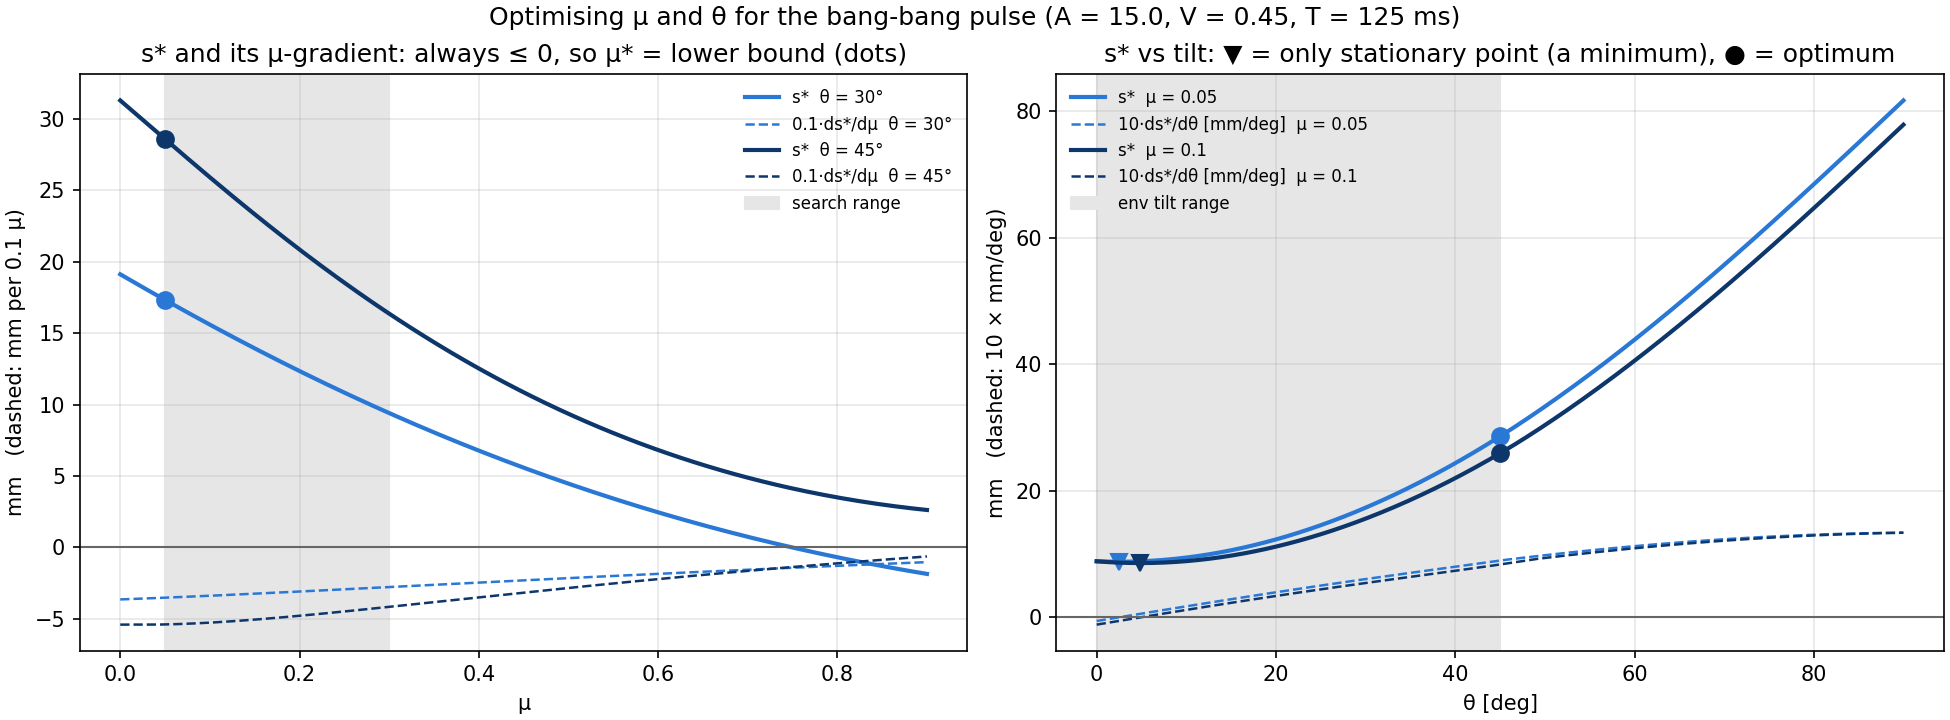
\includegraphics[width=\linewidth]{fig_mu_low_optimise.png}
  \caption{Left: $s^*(\mu)$ (solid) and $\partial s^*/\partial\mu$ (dashed) at $30^\circ$ and $45^\circ$. The gradient
  is negative everywhere, so the optimum (dots) is the lower bound. Right: $s^*(\theta)$ and $\partial s^*/\partial\theta$
  for $\mu=0.05,0.1$. The only stationary point (triangles) is a minimum, and the optimum (dots) is the $45^\circ$
  limit.}\label{fig:opt}
\end{figure}

\begin{figure}[p]
  \centering
  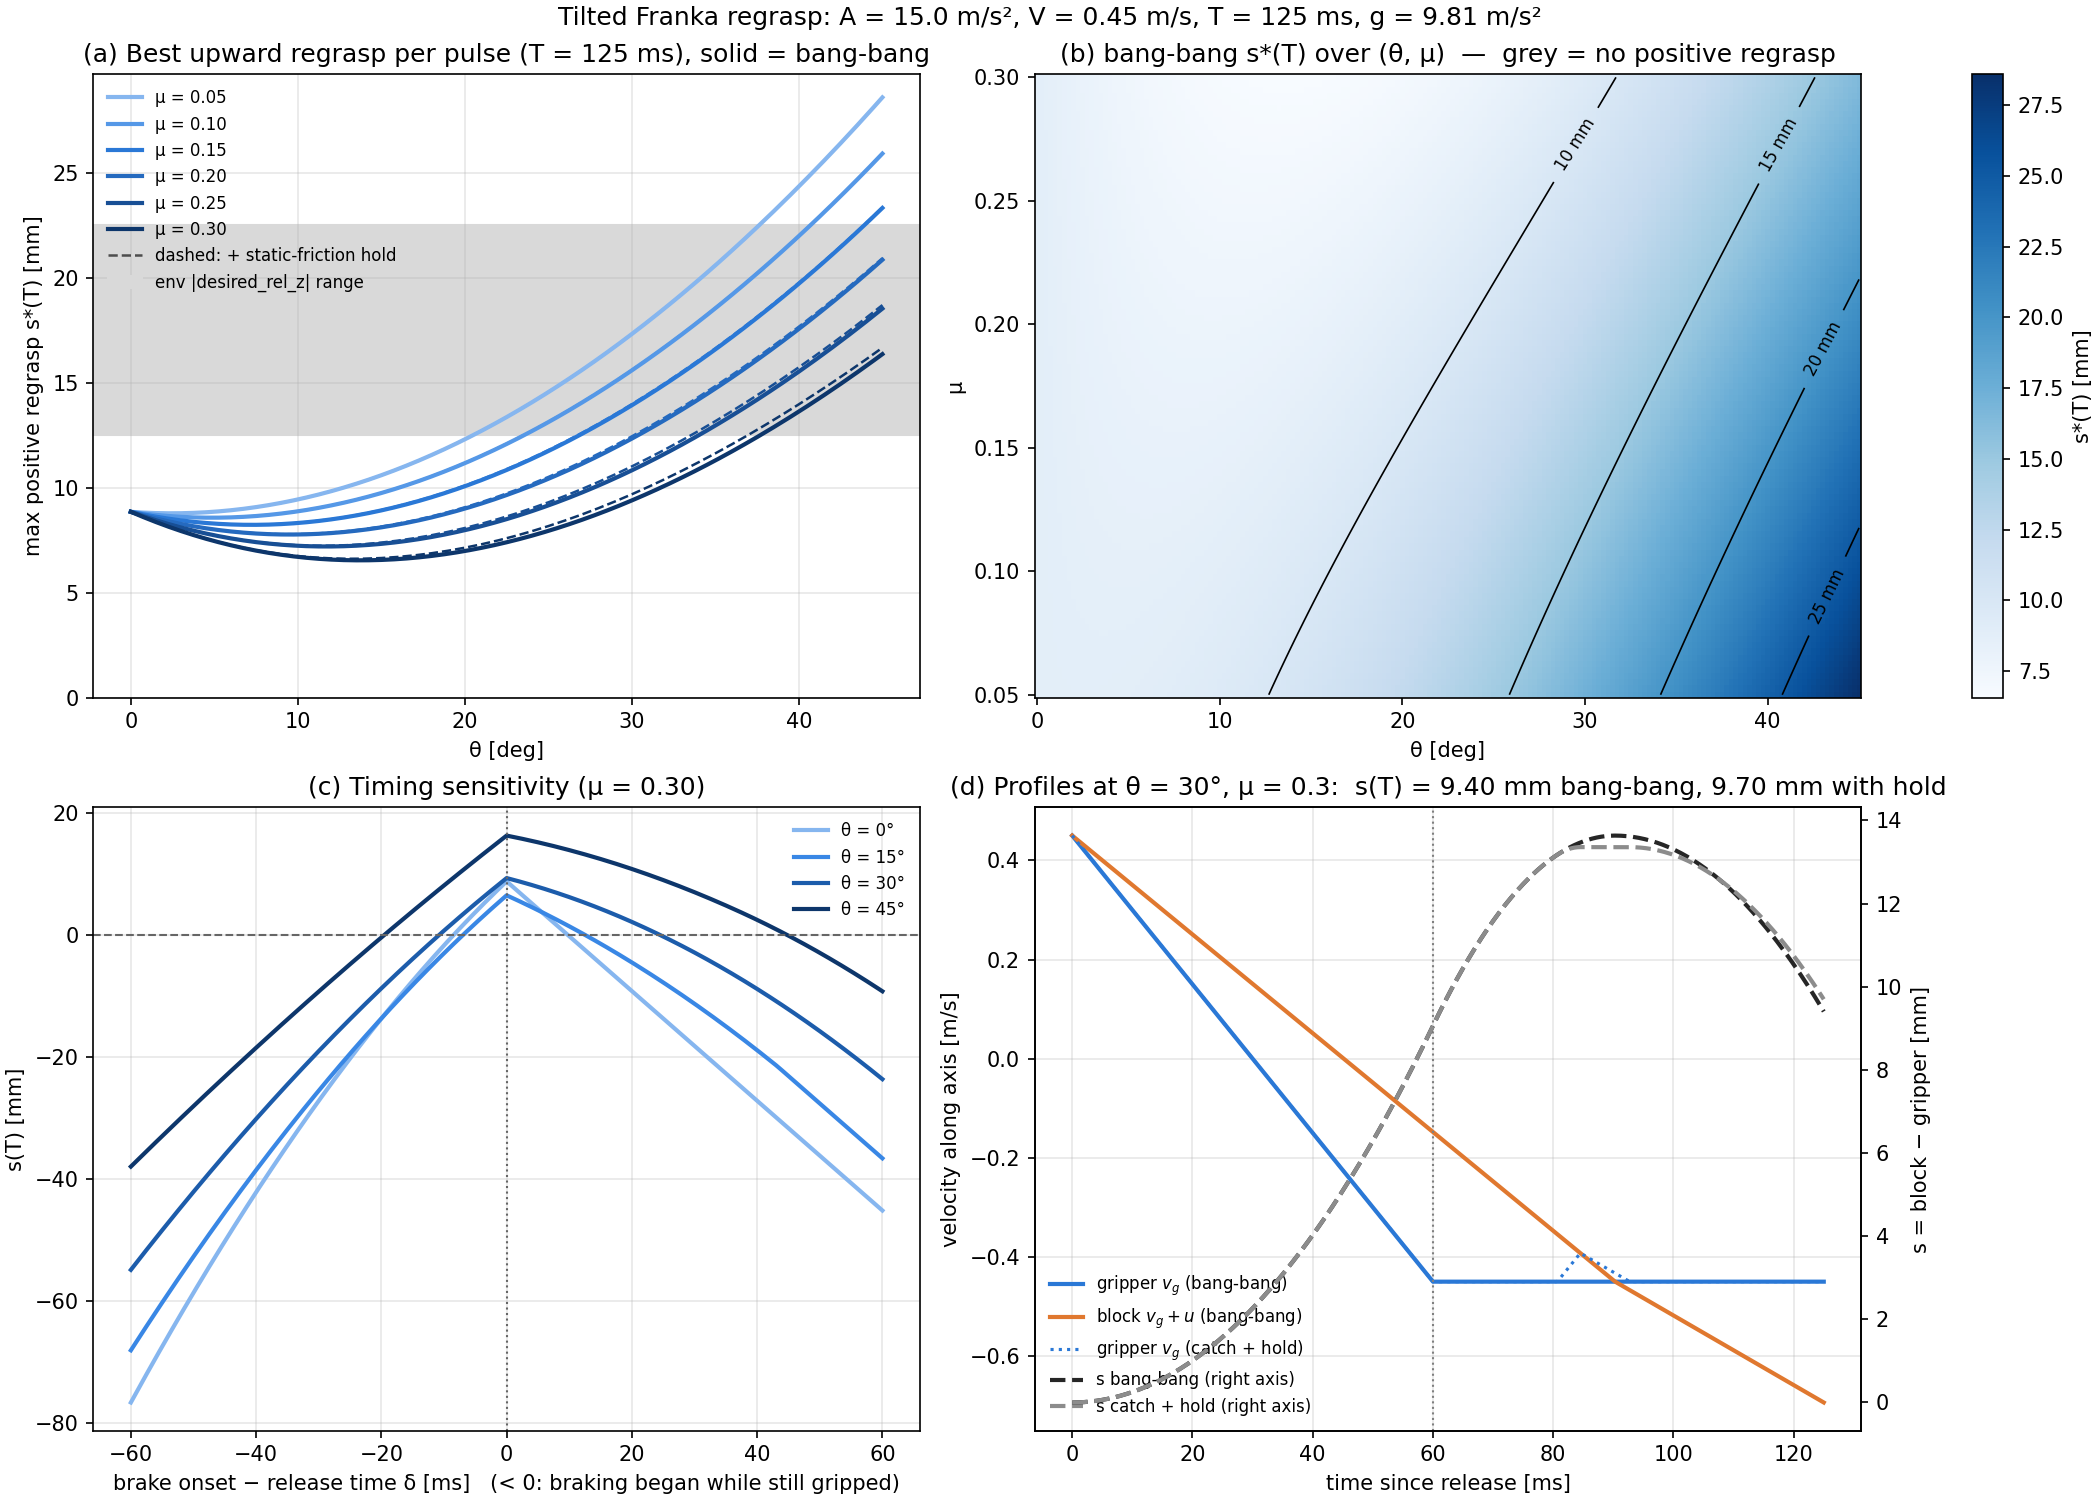
\includegraphics[width=\linewidth]{fig_mu_low.png}
  \caption{$\mu\in[0.05,0.3]$. (a) $s(T)$ vs.\ tilt (solid bang-bang, dashed with hold; grey band is the env target
  range). (b) Bang-bang map; grey would mean no positive regrasp. (c) Brake-onset timing. (d) Time traces at
  $\theta=30^\circ$, $\mu=0.3$.}
\end{figure}
\begin{figure}[p]
  \centering
  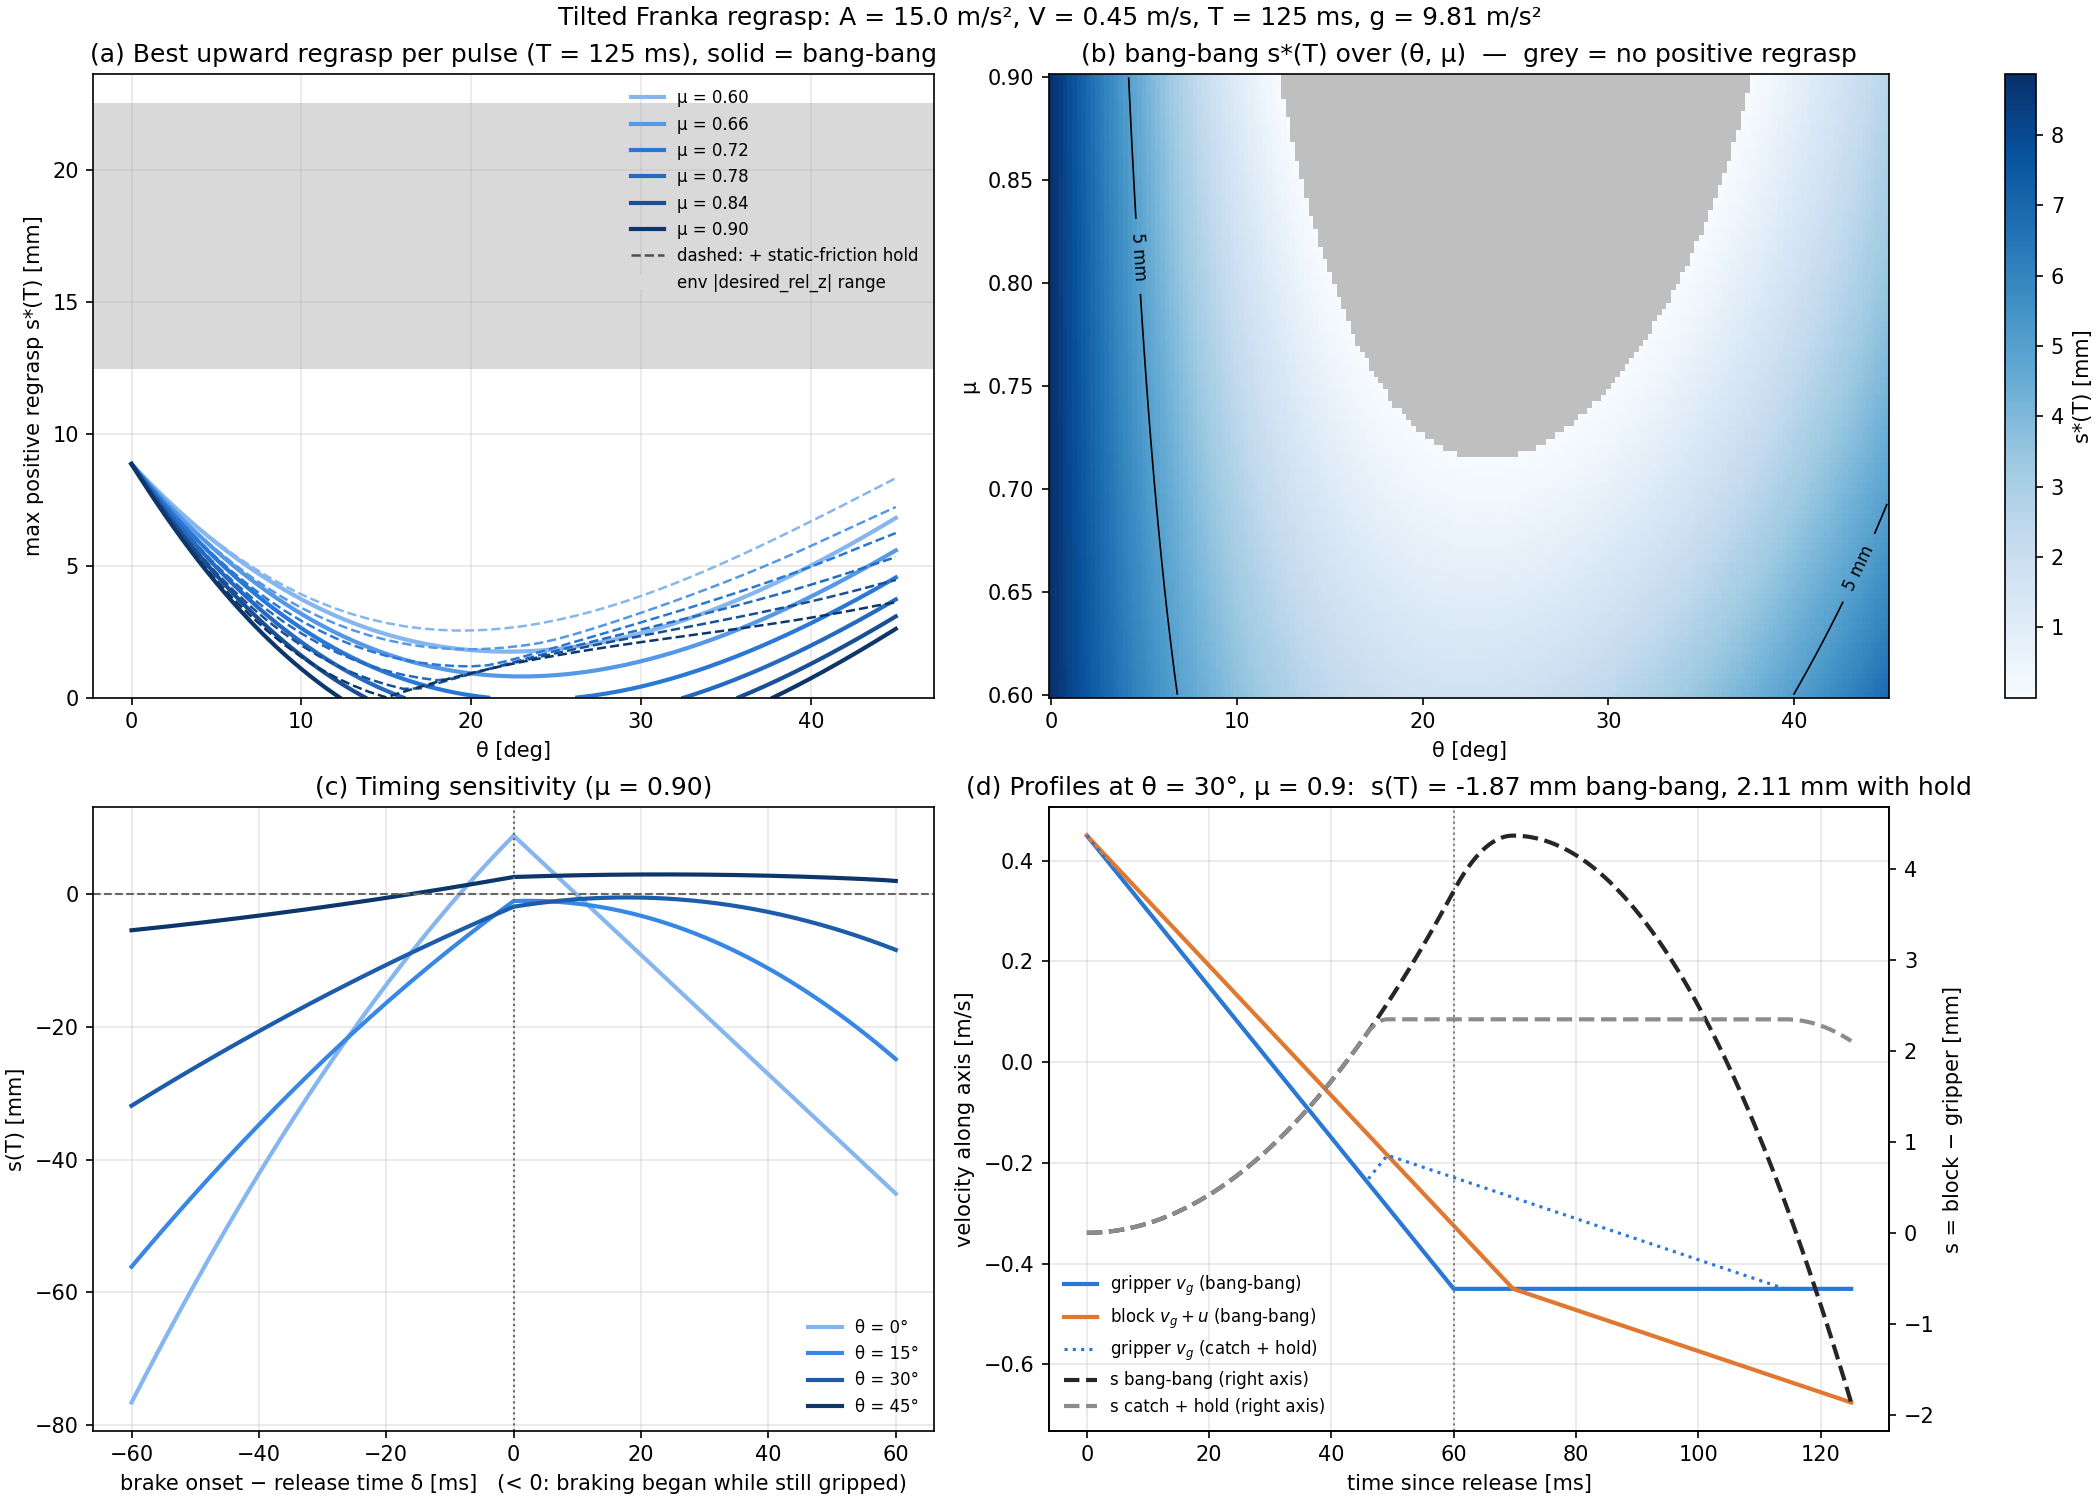
\includegraphics[width=\linewidth]{fig_mu_env.png}
  \caption{Same panels for the env friction range $\mu\in[0.6,0.9]$. The grey region in (b) is where bang-bang gives
  $s(T)\le0$. Panel (d) shows the long static-friction hold that makes $\theta=30^\circ$, $\mu=0.9$ positive again.}
\end{figure}


\section{Braking and reversing acceleration at $45^\circ$, $\mu=0.05$}\label{sec:accel}
Here $V=0.45$\,m/s, $T=125$\,ms, $\theta=45^\circ$ and $\mu=0.05$ are fixed, and the acceleration limit varies over
$[12,20]$\,m/s$^2$. The gripper reversal is split into two parts, each with its own limit:
\emph{braking} $+V\to0$ at $-A_{\rm b}$ (duration $V/A_{\rm b}$) and \emph{reversing} $0\to-V$ at $-A_{\rm r}$
(duration $V/A_{\rm r}$). The env's single \code{Z\_ACC\_MAX} is the diagonal $A_{\rm b}=A_{\rm r}=A$.
Proposition~\ref{prop:bb} still applies: while the block rises, the best gripper motion is the fastest allowed
reversal, and the free optimiser confirms this (below).

\paragraph{Closed form.} While the block rises, friction is the constant $-c$. Integrating
$\dot u=-a_g-g_a-c$ from $u(0)=0$ gives
\[
  u(t)=\big(V-v_g(t)\big)-b\,t,\qquad s(t)=\int_0^t\big(V-v_g\big)\,d\tau-\tfrac12 b\,t^2 .
\]
Once the gripper reaches $-V$, $u=2V-bt$, so the block peaks at
\[
  t_p=\frac{2V}{b}\qquad\text{(independent of }A_{\rm b},A_{\rm r}).
\]
Up to $t_p$ the integral equals $2Vt_p$ minus the \emph{reversal deficit}
\[
  D=\int_{\text{ramp}}\big(V+v_g\big)\,dt=\underbrace{\tfrac32\,V\cdot\tfrac{V}{A_{\rm b}}}_{\text{braking, }v_g:\,V\to0}
   +\underbrace{\tfrac12\,V\cdot\tfrac{V}{A_{\rm r}}}_{\text{reversing, }v_g:\,0\to-V}.
\]
The peak is at $s_p=2V^2/b-D$, and the block then falls at $d$ for the remaining $r=T-t_p$:
\begin{equation}
  \boxed{\ s^*=\frac{2V^2}{b}-\frac{3V^2}{2A_{\rm b}}-\frac{V^2}{2A_{\rm r}}-\tfrac12\,d\,(T-t_p)^2\ }
  \qquad(t_p<T,\ A_{\rm b},A_{\rm r}>b).
  \label{eq:ramp}
\end{equation}
With $A_{\rm b}=A_{\rm r}=A$ this reduces to $2V^2(1/b-1/A)-\tfrac12dr^2$, which is \eqref{eq:closed} again.
\begin{itemize}
  \item $2V^2/b=55.60$\,mm is the ideal of an \emph{instant} reversal ($A\to\infty$): the block gets relative speed
        $2V$ at once and coasts up against $b$.
  \item $D$ is what the finite reversal costs.
  \item At this tilt the fall term is negligible: $b=7.284$, $t_p=123.57$\,ms, $r=1.43$\,ms, $\tfrac12dr^2=0.007$\,mm.
        The pulse ends almost exactly at the peak.
\end{itemize}
\eqref{eq:ramp} matches the exact integrator to $10^{-17}$\,m over the whole $[12,20]^2$ grid.

\paragraph{Gradients.}
\[
  \frac{\partial s^*}{\partial A_{\rm b}}=\frac{3V^2}{2A_{\rm b}^2},\qquad
  \frac{\partial s^*}{\partial A_{\rm r}}=\frac{V^2}{2A_{\rm r}^2},\qquad
  \frac{d s^*}{dA}\Big|_{A_{\rm b}=A_{\rm r}}=\frac{2V^2}{A^2}.
\]
Both are positive and fall off as $1/A^2$. Braking is worth three times as much as reversing: each millisecond saved
while the gripper still moves \emph{up} is pure loss avoided, because at that point the block and gripper are still
moving apart slowly. With the same total "acceleration budget", $A_{\rm b}=20$, $A_{\rm r}=12$ gives 31.97\,mm,
while $A_{\rm b}=12$, $A_{\rm r}=20$ gives 25.22\,mm.

\begin{center}
\small
\begin{tabular}{c|ccc|cc|c}
\toprule
$A$ [m/s$^2$] & ramp $2V/A$ & $s^*$ [mm] & $ds^*/dA$ [mm/(m/s$^2$)] & 20\,ms steps & $s^*$, 20\,ms steps & optimiser\\
\midrule
12 & 75.0 ms & 21.85 & 2.81 & 3.75 & 21.40 & 21.85\\
13 & 69.2 ms & 24.44 & 2.40 & 3.46 & 23.80 & \\
14 & 64.3 ms & 26.67 & 2.07 & 3.21 & 26.20 & \\
15 & 60.0 ms & 28.60 & 1.80 & 3.00 & 28.60 & \\
16 & 56.2 ms & 30.29 & 1.58 & 2.81 & 29.80 & 30.27\\
17 & 52.9 ms & 31.77 & 1.40 & 2.65 & 31.00 & \\
18 & 50.0 ms & 33.10 & 1.25 & 2.50 & 32.20 & \\
19 & 47.4 ms & 34.28 & 1.12 & 2.37 & 33.40 & \\
20 & 45.0 ms & 35.35 & 1.01 & 2.25 & 34.60 & 35.35\\
\bottomrule
\end{tabular}
\end{center}
\noindent Notes on the table:
\begin{itemize}
  \item The static-friction hold adds $<0.001$\,mm here, because the block barely falls.
  \item The free optimiser (50 pieces of 2.5\,ms) cannot beat \eqref{eq:ramp}. At $A=16$ the 56.25\,ms ramp is not a
        multiple of its 2.5\,ms grid, which is why it lands 0.01\,mm lower.
  \item Going from $A=15$ to $20$ gains $+6.75$\,mm ($+24\%$). Going from 15 to 12 loses $6.75$\,mm.
\end{itemize}

\paragraph{The env's 20\,ms control steps.} The env limits $|\Delta v|\le A\Delta$ per 20\,ms step, so the reversal
is exact only when $2V/(A\Delta)$ is a whole number. That happens at $A=15$ (3 steps), and also at $11.25$ (4) and
$22.5$ (2). For other $A$ the last step can only be partial, the reversal is effectively slower, and $s^*$ drops by
0.4--0.8\,mm (column "with 20\,ms steps"; best is full steps first, the partial step last). Within $[12,20]$ the
env-quantised gain from 15 to 20 is therefore $+6.0$\,mm. The next exact point, $A=22.5$, would give
$2V^2(1/b-1/22.5)=37.6$\,mm.

\paragraph{What a higher $A$ requires.} The gripped block must follow the gripper's pre-release acceleration, which
needs $2\mu N\ge m(g\cos\theta+A)$. At $45^\circ$ and $\mu=0.05$ that is $N\ge6.6$\,N per finger at $A=12$,
$7.7$\,N at 15 and $9.4$\,N at 20. The arm must also actually deliver the acceleration along the tilted axis. The env's
feed-forward filter ($\omega_n=75$\,rad/s, $\zeta=0.33$) overshoots in proportion to $A$ (Section~\ref{sec:assump}).

\begin{figure}[h]
  \centering
  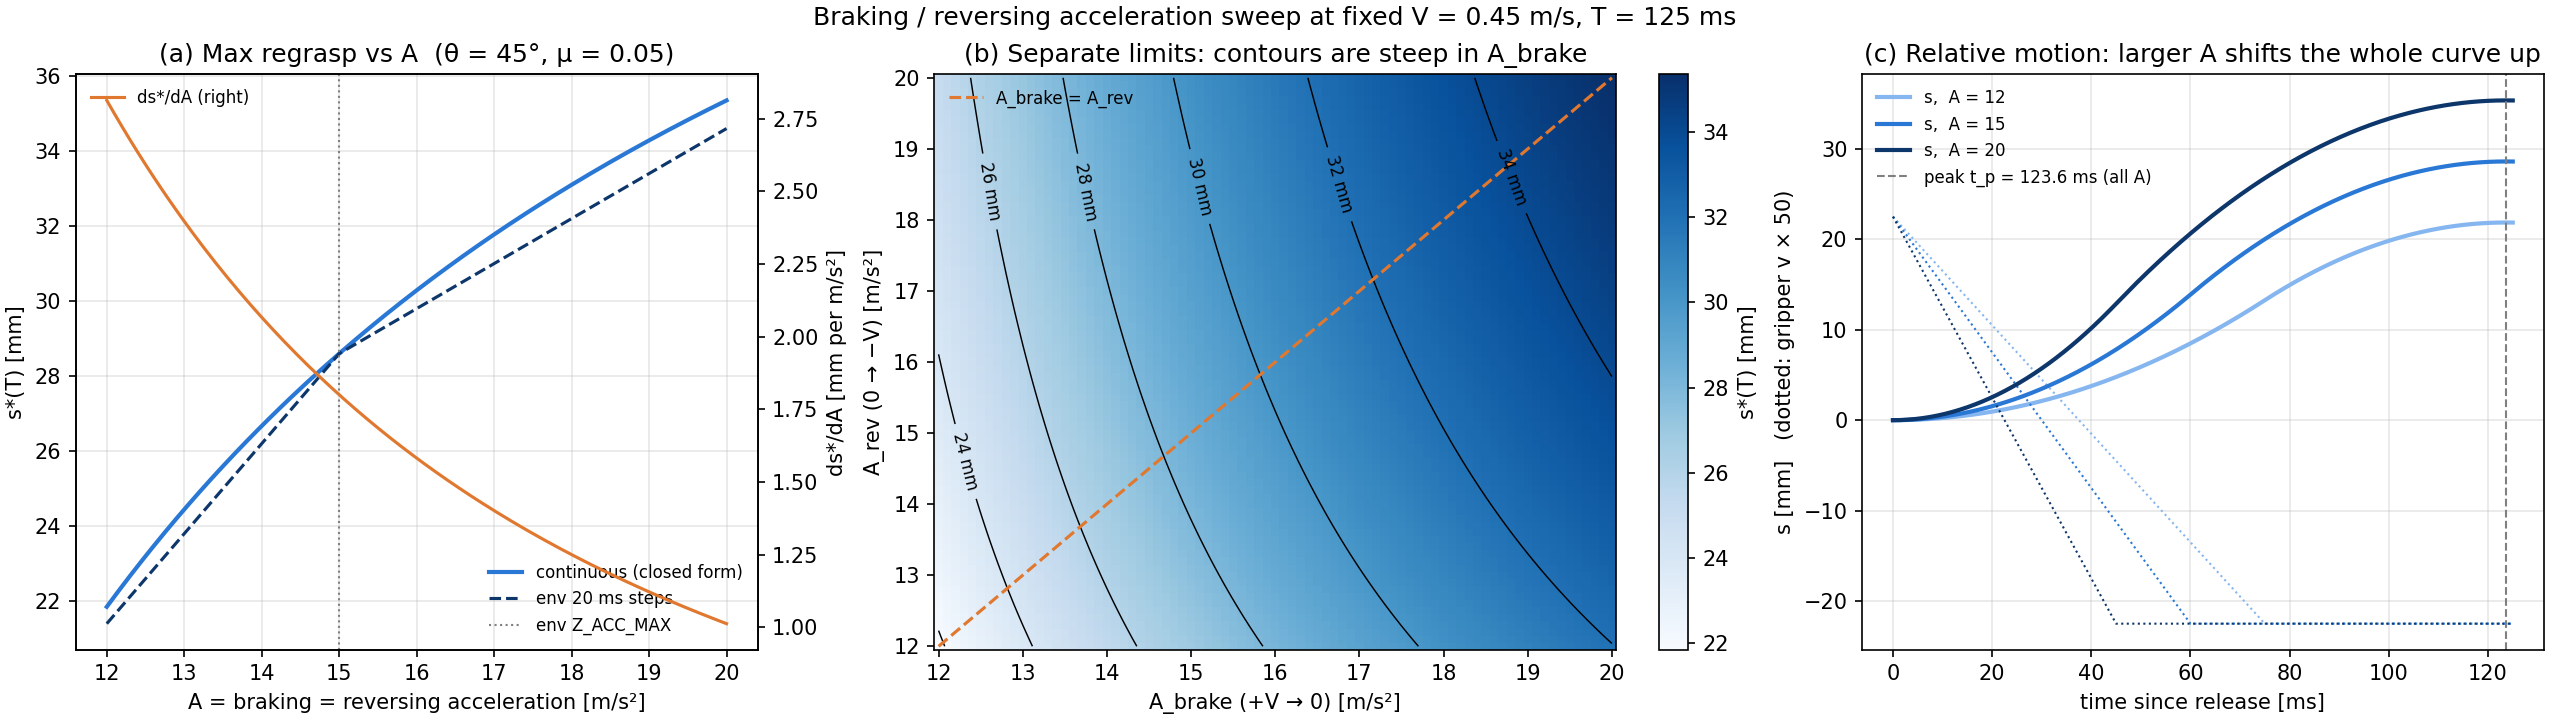
\includegraphics[width=\linewidth]{fig_accel.png}
  \caption{$\theta=45^\circ$, $\mu=0.05$, $V=0.45$\,m/s, $T=125$\,ms. (a) $s^*$ vs.\ $A$: continuous (solid) and with
  the env's 20\,ms steps (dashed), plus the marginal gain $2V^2/A^2$. (b) Separate braking/reversing limits: the
  contours run nearly parallel to the $A_{\rm r}$ axis because braking matters $3\times$ more. (c) Relative motion for
  $A=12,15,20$. All three peak at the same $t_p=2V/b$.}\label{fig:accel}
\end{figure}

\section{Assumptions to check against the simulator}\label{sec:assump}
\begin{enumerate}
  \item \textbf{The block rests on one finger while open} (normal load $mg\sin\theta$). This needs the fingers to open
        in the tilt plane, the same assumption as the earlier hand formula. If the tilt is across the finger
        faces instead, the block is not supported sideways and $c$ is not $\mu g\sin\theta$.
  \item \textbf{Ideal tracking.} The env filters the velocity feed-forward through
        $5625/(s^2+49.5s+5625)$, which is under-damped: acceleration peaks overshoot 15\,m/s$^2$ and lag by roughly
        10--20\,ms. The joint-space IK adds more lag. Treat the bang-bang value as an upper bound for this
        controller.
  \item \textbf{Instant release and regrasp}, with $T$ measured between the env's force thresholds. During finger
        closing the block may slip further if $u(T)\neq0$; in panel (d) $u(T)<0$, so any extra slip is downward.
  \item \textbf{Coulomb friction with $\mu_s=\mu_k$.} The hold phase sits \emph{exactly} on the static-friction limit.
        This is a theoretical bound: in practice use $a_g=-(1-\epsilon)k$ for margin, and expect soft contacts to creep.
  \item Torsional friction and rotation of the block are ignored.
\end{enumerate}

\section{Using the script}
\begin{verbatim}
python3 assess_angle.py                            # mu in [0.05, 0.3], T = 125 ms
python3 assess_angle.py --mu-min 0.6 --mu-max 0.9  # env friction range
python3 assess_angle.py --pulse 0.160              # other free time
python3 assess_angle.py --verify                   # optimiser check (~1-2 min)
python3 assess_angle.py --optimise                 # best mu and best theta
python3 assess_angle.py --accel-sweep              # A from 12 to 20 at 45 deg
\end{verbatim}
Main functions:
\begin{itemize}
  \item \code{relative\_motion}: the exact integrator of \eqref{eq:eom}.
  \item \code{closed\_form}: Eq.~\eqref{eq:closed}.
  \item \code{max\_positive\_regrasp}: the bang-bang value.
  \item \code{max\_positive\_regrasp\_hold}: the brake--catch--hold value.
  \item \code{onset\_profile}: the timing study.
  \item \code{verify\_optimum}: the free optimiser.
  \item \code{closed\_form\_gradients}, \code{gradient\_ascent}, \code{optimise\_report}: Section~\ref{sec:opt}.
  \item \code{closed\_form\_ramp}, \code{ramp\_profile}, \code{accel\_sweep\_report}: Section~\ref{sec:accel}.
\end{itemize}

\end{document}
